%Version 3.1 December 2024
% See section 11 of the User Manual for version history
%
%%%%%%%%%%%%%%%%%%%%%%%%%%%%%%%%%%%%%%%%%%%%%%%%%%%%%%%%%%%%%%%%%%%%%%
%%                                                                 %%
%% Please do not use \input{...} to include other tex files.       %%
%% Submit your LaTeX manuscript as one .tex document.              %%
%%                                                                 %%
%% All additional figures and files should be attached             %%
%% separately and not embedded in the \TeX\ document itself.       %%
%%                                                                 %%
%%%%%%%%%%%%%%%%%%%%%%%%%%%%%%%%%%%%%%%%%%%%%%%%%%%%%%%%%%%%%%%%%%%%%

%%\documentclass[referee,sn-basic]{sn-jnl}% referee option is meant for double line spacing

%%=======================================================%%
%% to print line numbers in the margin use lineno option %%
%%=======================================================%%

%%\documentclass[lineno,pdflatex,sn-basic]{sn-jnl}% Basic Springer Nature Reference Style/Chemistry Reference Style

%%=========================================================================================%%
%% the documentclass is set to pdflatex as default. You can delete it if not appropriate.  %%
%%=========================================================================================%%

%%\documentclass[sn-basic]{sn-jnl}% Basic Springer Nature Reference Style/Chemistry Reference Style

%%Note: the following reference styles support Namedate and Numbered referencing. By default the style follows the most common style. To switch between the options you can add or remove “Numbered” in the optional parenthesis. 
%%The option is available for: sn-basic.bst, sn-chicago.bst%  
 
%%\documentclass[pdflatex,sn-nature]{sn-jnl}% Style for submissions to Nature Portfolio journals
%%\documentclass[pdflatex,sn-basic]{sn-jnl}% Basic Springer Nature Reference Style/Chemistry Reference Style
%\documentclass[pdflatex,sn-mathphys-num]{sn-jnl}% Math and Physical Sciences Numbered Reference Style
\documentclass[pdflatex,lineno,referee,sn-vancouver-num]{sn-jnl}
%%\documentclass[pdflatex,sn-mathphys-ay]{sn-jnl}% Math and Physical Sciences Author Year Reference Style
%%\documentclass[pdflatex,sn-aps]{sn-jnl}% American Physical Society (APS) Reference Style
%%\documentclass[pdflatex,sn-vancouver-num]{sn-jnl}% Vancouver Numbered Reference Style
%%\documentclass[pdflatex,sn-vancouver-ay]{sn-jnl}% Vancouver Author Year Reference Style
%%\documentclass[pdflatex,sn-apa]{sn-jnl}% APA Reference Style
%%\documentclass[pdflatex,sn-chicago]{sn-jnl}% Chicago-based Humanities Reference Style

%%%% Standard Packages
%%<additional latex packages if required can be included here>

\usepackage{graphicx}%
\usepackage[utf8]{inputenc}%
\usepackage[T1]{fontenc}%
\usepackage[spanish,es-noshorthands,es-tabla]{babel}
\usepackage{multirow}%
\usepackage{amsmath,amssymb,amsfonts}%
\usepackage{amsthm}%
\usepackage{mathrsfs}%
\usepackage[title]{appendix}%
\usepackage{xcolor}%
\usepackage{textcomp}%
\usepackage{manyfoot}%
\usepackage{booktabs}%
\usepackage{algorithm}%
\usepackage{algorithmicx}%
\usepackage{algpseudocode}%
\usepackage{listings}%
\usepackage{tabularx}%
\usepackage{tikz}%
\usetikzlibrary{positioning,arrows.meta}%
\graphicspath{{figures/}{../reports/}}%
%%%%

%%%%%=============================================================================%%%%
%%%%  Remarks: This template is provided to aid authors with the preparation
%%%%  of original research articles intended for submission to journals published 
%%%%  by Springer Nature. The guidance has been prepared in partnership with 
%%%%  production teams to conform to Springer Nature technical requirements. 
%%%%  Editorial and presentation requirements differ among journal portfolios and 
%%%%  research disciplines. You may find sections in this template are irrelevant 
%%%%  to your work and are empowered to omit any such section if allowed by the 
%%%%  journal you intend to submit to. The submission guidelines and policies 
%%%%  of the journal take precedence. A detailed User Manual is available in the 
%%%%  template package for technical guidance.
%%%%%=============================================================================%%%%

%% as per the requirement new theorem styles can be included as shown below
\theoremstyle{thmstyleone}%
\newtheorem{theorem}{Theorem}%  meant for continuous numbers
%%\newtheorem{theorem}{Theorem}[section]% meant for sectionwise numbers
%% optional argument [theorem] produces theorem numbering sequence instead of independent numbers for Proposition
\newtheorem{proposition}[theorem]{Proposition}% 
%%\newtheorem{proposition}{Proposition}% to get separate numbers for theorem and proposition etc.

\theoremstyle{thmstyletwo}%
\newtheorem{example}{Example}%
\newtheorem{remark}{Remark}%

\theoremstyle{thmstylethree}%
\newtheorem{definition}{Definition}%

\lstdefinestyle{py}{
  language=Python,
  basicstyle=\ttfamily\footnotesize,
  keywordstyle=\color{blue!60!black}\bfseries,
  commentstyle=\color{green!40!black}\itshape,
  stringstyle=\color{red!60!black},
  frame=single,
  breaklines=true,
  columns=fullflexible,
  showstringspaces=false
}
\algrenewcommand\algorithmicrequire{\textbf{Entrada:}}

\raggedbottom
%%\unnumbered% uncomment this for unnumbered level heads

\begin{document}

\title[Elementos transponibles con perfiles de k-mers en MongoDB]{Almacenamiento y consulta de 239.946 secuencias de elementos transponibles con perfiles de k-mers en MongoDB}

%%=============================================================%%
%% GivenName	-> \fnm{Joergen W.}
%% Particle	-> \spfx{van der} -> surname prefix
%% FamilyName	-> \sur{Ploeg}
%% Suffix	-> \sfx{IV}
%% \author*[1,2]{\fnm{Joergen W.} \spfx{van der} \sur{Ploeg} 
%%  \sfx{IV}}\email{iauthor@gmail.com}
%%=============================================================%%
\author*[1]{\fnm{Alejandro} \sur{Diaz}}\email{alejo.diaz.ruiz@gmail.com}

\author*[1]{\fnm{Sebastian} \sur{Villaneda}}\email{sebastianvillaneda202@gmail.com}

\author*[1]{\fnm{Johan} \sur{Javier}}\email{johanjavier654@gmail.com}

\author*[1]{\fnm{Juan Sebastian} \sur{Lopez}}\email{juanse150906@gmail.com}

\affil*[1]{\orgdiv{Ingeniería de Sistemas}, \orgname{Universidad Autónoma de Manizales}, \orgaddress{\city{Manizales}, \state{Caldas}, \country{Colombia}}}

%%==================================%%
%% Sample for unstructured abstract %%
%%==================================%%

\abstract{Los elementos transponibles (TE) son secuencias de ADN móviles que constituyen una fracción muy grande de muchos genomas eucariotas. Su análisis computacional, en particular la clasificación automática con aprendizaje de máquina, depende de repositorios grandes y heterogéneos y de perfiles de k-mers como atributos de entrada. Almacenar esos perfiles junto con la taxonomía y las métricas de calidad plantea un problema de modelado y de escala. En este trabajo se diseña, se implementa y se evalúa un modelo documental en MongoDB para PanTEon Database v1.6.1, que reúne 239.946 secuencias de 2.790 especies (963.901.415 bases). Se desarrolló un \emph{pipeline} en Python que lee el FASTA en \emph{streaming}, limpia y normaliza el CSV taxonómico, cruza ambas fuentes con una llave normalizada de especie, calcula las métricas de calidad y los perfiles de k-mers de $k=1$ a $k=6$, y carga los datos por lotes y de forma reanudable. El modelo híbrido propuesto referencia la taxonomía desde una colección de especies y embebe las métricas y los k-mers en cada secuencia. Está protegido por validadores \texttt{\$jsonSchema} estrictos y por índices estratégicos. La carga se verificó contra el FASTA original sin discrepancias ni rechazos. Con una muestra de 20.000 secuencias se compararon dos estrategias de almacenamiento: k-mers embebidos (A) frente a k-mers en una colección separada (B). Los k-mers representan cerca del 90\,\% del tamaño de cada documento (unos 26 de 29 KB). La estrategia B aceleró un 23\,\% las agregaciones que no usan k-mers, mientras que la A fue más rápida al recuperar el perfil de k-mers junto con su taxonomía (0,43 ms frente a 0,77 ms). Sobre la base completa, las consultas con índice respondieron en 0,35--0,37 ms, frente a 117--153 ms con recorrido completo de la colección. Se discuten las limitaciones del diseño, las amenazas a la validez derivadas de la calidad de las fuentes y una ruta de crecimiento basada en fragmentación (\emph{sharding}). Los resultados indican que una base de datos orientada a documentos es una opción competitiva para gestionar bibliotecas moleculares complejas.}

%%================================%%
%% Sample for structured abstract %%
%%================================%%

% \abstract{\textbf{Purpose:} The abstract serves both as a general introduction to the topic and as a brief, non-technical summary of the main results and their implications. The abstract must not include subheadings (unless expressly permitted in the journal's Instructions to Authors), equations or citations. As a guide the abstract should not exceed 200 words. Most journals do not set a hard limit however authors are advised to check the author instructions for the journal they are submitting to.
% 
% \textbf{Methods:} The abstract serves both as a general introduction to the topic and as a brief, non-technical summary of the main results and their implications. The abstract must not include subheadings (unless expressly permitted in the journal's Instructions to Authors), equations or citations. As a guide the abstract should not exceed 200 words. Most journals do not set a hard limit however authors are advised to check the author instructions for the journal they are submitting to.
% 
% \textbf{Results:} The abstract serves both as a general introduction to the topic and as a brief, non-technical summary of the main results and their implications. The abstract must not include subheadings (unless expressly permitted in the journal's Instructions to Authors), equations or citations. As a guide the abstract should not exceed 200 words. Most journals do not set a hard limit however authors are advised to check the author instructions for the journal they are submitting to.
% 
% \textbf{Conclusion:} The abstract serves both as a general introduction to the topic and as a brief, non-technical summary of the main results and their implications. The abstract must not include subheadings (unless expressly permitted in the journal's Instructions to Authors), equations or citations. As a guide the abstract should not exceed 200 words. Most journals do not set a hard limit however authors are advised to check the author instructions for the journal they are submitting to.}

\keywords{k-mers, MongoDB, bases de datos NoSQL, PanTEon, pipeline de datos, evaluación de rendimiento, integridad de datos, elementos transponibles}

%%\pacs[JEL Classification]{D8, H51}

%%\pacs[MSC Classification]{35A01, 65L10, 65L12, 65L20, 65L70}

\maketitle

\section{Introducción}\label{sec:intro}

Los elementos transponibles (TE, del inglés \emph{transposable elements}) son secuencias de ADN capaces de moverse o copiarse dentro del genoma. En muchos organismos, sobre todo en plantas, constituyen la fracción dominante del material genético, en algunos casos por encima del 80\,\%, y participan en la regulación génica y en la evolución de los genomas. El sistema de clasificación más usado los agrupa de forma jerárquica en clases, órdenes y superfamilias \cite{wicker2007}. La clase I reúne los retrotransposones, que se copian a través de un intermediario de ARN, y la clase II reúne los transposones de ADN, que se escinden y se insertan directamente.

La anotación de los TE en los genomas que se secuencian cada año ya no puede hacerse a mano, por lo que se ha recurrido a clasificadores automáticos basados en aprendizaje de máquina. Muchos de ellos describen cada secuencia mediante las frecuencias de sus k-mers, es decir, de todas las subcadenas de longitud $k$. PASTEC, por ejemplo, entrena máquinas de soporte vectorial con frecuencias de tetrámeros y pentámeros \cite{hoede2014pastec}, y DeepTE alimenta una red neuronal convolucional con conteos de k-mers \cite{yan2020deepte}. PanTEon es un marco que combina una base de datos armonizada con una plataforma abierta para evaluar este tipo de clasificadores en animales, plantas y hongos \cite{orozco2026panteon}, y su versión 1.6.1 reúne casi 240.000 secuencias \cite{orozco2026panteondb}.

Trabajar con una colección de este tamaño plantea varios problemas de ingeniería de datos. Las secuencias y su taxonomía llegan en archivos distintos (un FASTA de cerca de 964 millones de bases y un CSV con las especies) que nombran las mismas entidades de forma diferente. Cada secuencia genera además un perfil de k-mers de $k=1$ a $k=6$, que puede tener hasta 5460 atributos, y ese perfil termina pesando mucho más que la propia secuencia. Hay que decidir, por tanto, cómo relacionar taxonomía y secuencias, dónde guardar los k-mers, cómo impedir que entren datos inválidos y qué índices evitan recorrer toda la colección en cada consulta.

El objetivo de este trabajo es diseñar, implementar y evaluar un modelo documental en MongoDB para almacenar y consultar PanTEon Database v1.6.1 con sus perfiles de k-mers. Las contribuciones son cuatro:
\begin{itemize}
  \item un \emph{pipeline} reproducible en Python que lee, limpia, cruza y carga las 239.946 secuencias y 2.790 especies, y que se verificó contra el FASTA original;
  \item un modelo híbrido de dos colecciones, con validación estricta mediante \texttt{\$jsonSchema} e índices estratégicos;
  \item una comparación experimental entre guardar los k-mers dentro de cada secuencia y guardarlos en una colección aparte, junto con la medición del efecto de los índices;
  \item un análisis de las limitaciones del diseño, de las amenazas a la validez asociadas a la calidad de las fuentes y de la forma de escalar la solución si los datos crecieran.
\end{itemize}

El resto del documento se organiza así. La Sección~\ref{sec:relacionado} revisa cómo otros recursos organizan esta información. La Sección~\ref{sec:metodos} describe los datos, el modelo, el \emph{pipeline} y el diseño de los experimentos. La Sección~\ref{sec:resultados} presenta los resultados y su discusión, y la Sección~\ref{sec:conclusiones} cierra con las conclusiones.

\section{Trabajo relacionado}\label{sec:relacionado}

\paragraph{Repositorios de elementos transponibles.} Repbase ha sido durante años la referencia curada manualmente de secuencias repetitivas eucariotas \cite{bao2015repbase}, y su acceso está sujeto a registro y a condiciones de licencia. Dfam es una base de acceso abierto que distribuye familias de TE como secuencias consenso y modelos de Markov ocultos de perfil, junto con anotaciones de genomas \cite{storer2021dfam}. Ambos recursos se distribuyen principalmente como archivos de texto (FASTA, formatos de modelos y de anotación) y se consultan por especie, familia o clasificación.

\paragraph{PanTEon.} PanTEon Database reúne TE de animales, plantas y hongos con un proceso de curación automática, un identificador estandarizado para cada secuencia y una edición de referencia para comparar clasificadores de forma justa \cite{orozco2026panteon,orozco2026panteondb}. Parte de sus secuencias proviene de Dfam, y las demás se integran mediante el propio marco. La base se distribuye en Zenodo como un archivo FASTA y un CSV con la taxonomía de cada especie, y el propósito de PanTEon es entrenar y evaluar modelos, no ofrecer un servicio de consulta.

\paragraph{Clasificadores basados en k-mers.} Herramientas como PASTEC \cite{hoede2014pastec} y DeepTE \cite{yan2020deepte} usan frecuencias de k-mers como atributos de entrada. En estos flujos, los k-mers se calculan a partir del FASTA cada vez que se entrena o se clasifica. Los perfiles no se guardan en una estructura que se pueda consultar, filtrar por taxonomía o validar.

\paragraph{Posición de este trabajo.} Hasta donde sabemos, ninguno de los recursos anteriores distribuye perfiles de k-mers precalculados ni un modelo de datos consultable que relacione secuencias, métricas de calidad y taxonomía con validación de integridad. Este trabajo aborda ese hueco sobre PanTEon Database v1.6.1. Se usa MongoDB, una base de datos orientada a documentos que permite validar la estructura con \texttt{\$jsonSchema}, anidar subdocumentos y analizar los planes de ejecución con \texttt{explain} \cite{mongodb2026docs}. Frente a la distribución en archivos planos, la base permite agregaciones, filtros combinados y exportaciones parametrizadas sin recorrer el FASTA completo.

\section{Materiales y métodos}\label{sec:metodos}

\begingroup
\sloppy % evita que los nombres en \texttt se salgan del margen

\subsection{Datos y problemas de calidad}\label{subsec:datos}

Se trabajó con la versión 1.6.1 de PanTEon, obtenida de Zenodo \cite{orozco2026panteondb}, que se distribuye en dos archivos:

\begin{itemize}
  \item \texttt{PanTEon\_Database\_v1.6.1.fasta}: 239.946 secuencias de elementos transponibles (TE), con un total de 963.901.415 bases. El encabezado de cada registro contiene el identificador de la secuencia, la clasificación del TE en tres niveles (clase, orden y superfamilia; por ejemplo \texttt{CLASSII} y \texttt{HELITRON}) y el nombre de la especie de origen. Se encontraron 66 cadenas de clasificación distintas.
  \item \texttt{PanTEon\_Database\_metadata\_v1.6.1.csv}: 2.790 especies con su taxonomía y el origen de su biblioteca de TE. Se conservaron las nueve columnas del archivo: \texttt{Kingdom}, \texttt{Phylum}, \texttt{Class}, \texttt{Order}, \texttt{Family}, \texttt{Species}, \texttt{Source}, \texttt{Source 2} y \texttt{Notes}.
\end{itemize}

Las dos fuentes usan los nombres \emph{Class} y \emph{Order} con significados distintos. En el CSV designan la clase y el orden taxonómicos del organismo (por ejemplo, \textit{Chromadorea} y \textit{Rhabditida}); en el FASTA, la clase y el orden del elemento transponible. Para evitar confusiones, los campos del TE se nombraron con el prefijo \texttt{te\_} (\texttt{te\_class}, \texttt{te\_order}, \texttt{te\_superfamily}) y los de la especie conservaron su nombre original dentro de su propia colección.

El procesamiento se hizo en Python 3.13 con pandas 3.1.0, NumPy 2.5.4, Biopython 1.88 \cite{cock2009biopython} y PyMongo 4.19.0, sobre una instancia local de MongoDB (\texttt{mongodb://localhost:27017}).

\paragraph{Lectura y validación del FASTA.} El FASTA se leyó en \emph{streaming} con \texttt{Bio.SeqIO.parse}, registro por registro, sin cargar el archivo completo en memoria. Para cada registro se separaron los campos del encabezado (identificador, clasificación original, clase, orden y superfamilia del TE y especie) y se validó la secuencia en tres aspectos:

\begin{enumerate}
  \item \textbf{Alfabeto.} La secuencia se pasa a mayúsculas y se comprueba que solo contenga A, C, G, T y N (función \texttt{normalizar\_secuencia}); cualquier otro símbolo genera un error. La exploración previa no encontró ningún carácter fuera de este alfabeto, de modo que no fue necesario decidir cómo tratar los códigos IUPAC ambiguos (R, Y, K\ldots).
  \item \textbf{Bases indeterminadas.} Se contó el número de N por secuencia y su porcentaje sobre la longitud. En total hay 2.147.161 N, y la secuencia con mayor proporción tiene un 50\,\% de N.
  \item \textbf{Longitud.} Se registró la longitud de cada secuencia y se calcularon el mínimo, la mediana y el máximo para detectar valores atípicos.
\end{enumerate}

También se revisaron los identificadores: 208.346 siguen el patrón \texttt{PDB} seguido de dígitos y 31.600 usan el nombre de la fuente (por ejemplo, \texttt{PumCon-1.11}). Ambos formatos son válidos, por lo que el esquema solo exige que el identificador sea una cadena no vacía y única.

\paragraph{Limpieza del CSV.} El CSV se leyó con todas las columnas como texto (\texttt{dtype=str}) y con \texttt{keep\_default\_na=False}, para que pandas no convirtiera por su cuenta cadenas como \texttt{NA} en valores nulos. La función \texttt{limpiar\_csv} aplica los siguientes pasos:

\begin{enumerate}
  \item Comprueba que existan las nueve columnas y descarta las demás.
  \item Elimina los espacios en los extremos de cada valor y convierte las cadenas vacías en \texttt{None}, que MongoDB guarda como \texttt{null}.
  \item Convierte en \texttt{None} los \emph{marcadores de faltante} de las columnas taxonómicas: textos que el CSV usa para decir que no hay dato. Se detectan con la expresión regular \verb|(?i)^no\b|, que reconoce cadenas que empiezan por la palabra \emph{no} sin afectar a nombres reales como \textit{Nostocales}. Solo aparecieron en \texttt{Order} (Tabla~\ref{tab:marcadores}).
  \item Separa la columna \texttt{Source 2}, que mezclaba dos tipos de información: los nombres de fuente (\texttt{Repbase}, \texttt{Dfam}) pasan a \texttt{source\_2} y el resto de los textos, a \texttt{annotation}.
  \item Verifica que \texttt{Species} no tenga vacíos y genera la llave de cruce \texttt{species\_key} sin modificar el nombre original.
\end{enumerate}

\begin{table}[htbp]
  \centering
  \caption{Marcadores de faltante encontrados en la columna \texttt{Order} y convertidos en \texttt{null}.}
  \label{tab:marcadores}
  \begin{tabular}{lr}
    \toprule
    Texto en el CSV & Apariciones \\
    \midrule
    \texttt{No trobat} & 7 \\
    \texttt{No order} & 5 \\
    \texttt{No ordre NCBI} & 2 \\
    \texttt{No Orden No trobat} & 2 \\
    \texttt{No ordre NCBI Caenogastropoda incertae sedis} & 1 \\
    \texttt{No order (eupecaria incertae sedis)} & 1 \\
    \texttt{No order Dothideomycetes incertae sedis} & 1 \\
    \midrule
    Total & 19 \\
    \bottomrule
  \end{tabular}
\end{table}

En tres de esos registros el marcador iba acompañado de la nota \textit{incertae sedis}, que indica que el taxón no tiene una posición clara. Esa nota se pierde en la base de datos, aunque se conserva en el CSV original. Tras la limpieza, los valores nulos por columna quedaron así: \texttt{Phylum} 3, \texttt{Class} 49, \texttt{Order} 48 (29 vacíos y 19 marcadores) y \texttt{Family} 76. \texttt{Kingdom} no tiene nulos y solo toma tres valores: Fungi (1.559), Animalia (780) y Plantae (451).

\paragraph{Cruce entre FASTA y CSV.} Las dos fuentes se relacionan por el nombre de la especie, pero no siempre lo escriben igual. Por eso se definió una llave de cruce con la función \texttt{clave}, que se aplica de la misma forma a ambas fuentes: elimina los espacios de los extremos, pasa a minúsculas, quita los puntos y colapsa los espacios internos repetidos:
\[
  \texttt{species\_key} = \text{colapsar}\bigl(\text{sin\_puntos}(\text{minúsculas}(\text{strip}(\texttt{Species})))\bigr).
\]
Antes de normalizar había 4 especies del FASTA sin metadatos en el CSV y 4 especies del CSV sin secuencias en el FASTA. Después de normalizar, ambas cifras quedaron en 0. El detalle se guardó en \texttt{reports/reporte\_cruce.csv}.

\subsection{Modelo de datos}\label{subsec:modelo}

MongoDB permite relacionar datos de dos maneras: \emph{embebiendo} un documento dentro de otro o \emph{referenciándolo} desde otra colección. El modelo adoptado combina ambas, y por eso se denomina híbrido (Figura~\ref{fig:modelo}):

\begin{itemize}
  \item \textbf{Referencia entre especies y secuencias.} Hay dos colecciones, \texttt{species} (2.790 documentos) y \texttt{sequences} (239.946 documentos), unidas en una relación 1:N mediante \texttt{species\_key}. La consulta conjunta se resuelve con \texttt{\$lookup}.
  \item \textbf{Embebido de métricas y k-mers.} Cada documento de \texttt{sequences} contiene sus métricas (subdocumento \texttt{metrics}) y sus conteos de k-mers (subdocumento \texttt{kmers}), porque siempre se consultan junto con la secuencia a la que pertenecen.
\end{itemize}

\begin{figure}[htbp]
  \centering
  \begin{tikzpicture}[
      font=\footnotesize,
      caja/.style={draw, rounded corners, align=left, inner sep=5pt, text width=4.7cm, anchor=north}]
    \node[caja] (sp) {\textbf{species} (2.790)\\[2pt]
      \texttt{species\_key} (único)\\
      \texttt{Species}\\
      \texttt{Kingdom}, \texttt{Phylum}, \texttt{Class},\\
      \texttt{Order}, \texttt{Family}\\
      \texttt{Source}, \texttt{source\_2},\\
      \texttt{annotation}, \texttt{Notes}};
    \node[caja, right=2.4cm of sp.north east, anchor=north west] (sq) {\textbf{sequences} (239.946)\\[2pt]
      \texttt{sequence\_id} (único)\\
      \texttt{species\_key}, \texttt{species\_raw}\\
      \texttt{te\_class}, \texttt{te\_order},\\
      \texttt{te\_superfamily}, \texttt{classification\_raw}\\
      \texttt{sequence}\\
      \texttt{metrics} \{\texttt{length}, \texttt{gc\_content},\\
      \quad\texttt{n\_count}, \texttt{n\_pct}\} \emph{(embebido)}\\
      \texttt{kmers} \{\texttt{k1} \ldots \texttt{k6}\} \emph{(embebido)}};
    \draw[{Bar}-{Latex}, thick] (sp.east) -- (sp.east -| sq.west) node[midway, above, font=\scriptsize]{1 : N} node[midway, below, font=\scriptsize]{\texttt{species\_key}};
  \end{tikzpicture}
  \caption{Modelo de datos híbrido: las especies se referencian desde las secuencias y las métricas y los k-mers se embeben en cada secuencia.}
  \label{fig:modelo}
\end{figure}

\paragraph{Representación de los k-mers.} Para cada secuencia se cuentan los k-mers de longitud $k=1,\dots,6$. El número de k-mers posibles es
\[
  \sum_{k=1}^{6} 4^k = 4 + 16 + 64 + 256 + 1024 + 4096 = 5460.
\]
El conteo se hace sobre un arreglo de NumPy de $4^k$ posiciones en orden alfabético (función \texttt{contar\_kmers}). Luego, \texttt{np.flatnonzero} selecciona solo las posiciones con conteo mayor que cero, que se traducen a su texto (\texttt{AA}, \texttt{AC}\ldots) y se guardan como enteros nativos de Python, ya que PyMongo no admite \texttt{numpy.int64}. Las ventanas que contienen al menos una N se descartan, porque no representan un k-mer conocido. El resultado tiene esta forma:
\begin{lstlisting}[style=py]
"kmers": {"k1": {"A": 120, "C": 85, ...},
          ...,
          "k6": {"AAAAAA": 3, "AAAAAC": 1, ...}}
\end{lstlisting}
En la muestra de 20.000 secuencias de la evaluación experimental (Sección~\ref{subsec:evaluacion}), los k-mers ocuparon cerca del 90\,\% del tamaño de cada documento, unos 26,26 KB de los 29,13 KB que pesa en promedio.

\paragraph{Métricas adicionales.} Además de los k-mers, cada secuencia guarda cuatro atributos: la longitud, el número de N, el porcentaje de N y el contenido de GC, calculado solo sobre las bases conocidas:
\[
  \mathrm{GC} = \frac{G + C}{A + C + G + T} \times 100.
\]

\paragraph{Validación e índices.} Ambas colecciones tienen un validador \texttt{\$jsonSchema} estricto. \texttt{Kingdom}, \texttt{source\_2} y \texttt{Notes} solo aceptan los valores de una lista cerrada (\texttt{enum}); \texttt{Phylum}, \texttt{Class}, \texttt{Order} y \texttt{Family} admiten \texttt{null}; \texttt{gc\_content} y \texttt{n\_pct} deben estar entre 0 y 100. Se crearon ocho índices:
\begin{itemize}
  \item en \texttt{species}: \texttt{species\_key} (único), (\texttt{Kingdom}, \texttt{Class}) y \texttt{Source};
  \item en \texttt{sequences}: \texttt{sequence\_id} (único), (\texttt{species\_key}, \texttt{te\_superfamily}), (\texttt{te\_class}, \texttt{te\_order}, \texttt{te\_superfamily}), \texttt{metrics.length} y \texttt{metrics.gc\_content}.
\end{itemize}

Una prueba con tres especies y 290 secuencias detectó que el primer esquema era demasiado restrictivo: rechazó 1 de 3 especies (por taxonomía vacía) y 39 de 290 secuencias (por exigir el prefijo \texttt{PDB} en el identificador). Tras corregir el esquema como se describe arriba, la misma prueba cargó todos los documentos sin rechazos.

\subsection{Decisiones de diseño}\label{subsec:decisiones}

La Tabla~\ref{tab:decisiones} resume las decisiones de diseño y la alternativa que se descartó en cada caso.

\begin{table}[htbp]
  \centering
  \caption{Decisiones del modelo de datos y alternativas descartadas.}
  \label{tab:decisiones}
  \begin{tabularx}{\linewidth}{>{\raggedright\arraybackslash}p{3.1cm} >{\raggedright\arraybackslash}p{3.1cm} X}
    \toprule
    Decisión & Alternativa descartada & Motivo \\
    \midrule
    Dos colecciones referenciadas & Embeber las secuencias en cada especie &
      Una especie con miles de secuencias, cada una con sus k-mers, superaría el límite de 16~MB por documento de MongoDB; además, la taxonomía se repetiría 239.946 veces si se hiciera al revés. \\
    K-mers embebidos en \texttt{sequences} & Colección aparte de k-mers &
      Los k-mers se leen siempre junto con su secuencia y así se evita un \texttt{\$lookup} por consulta. La comparación con la alternativa se presenta en la Sección~\ref{subsec:evaluacion}. \\
    Diccionario disperso & Arreglo denso de 5460 posiciones &
      En secuencias cortas, la mayoría de los 4096 k-mers posibles de $k=6$ tienen conteo 0. \\
    Conteos enteros & Frecuencias relativas &
      Las frecuencias se derivan del conteo y de la longitud. \\
    Prefijo \texttt{te\_} & Repetir \texttt{Class} y \texttt{Order} &
      Distingue la clasificación del TE de la taxonomía de la especie. \\
    Sin k-mers canónicos & Fusionar con el complemento inverso &
      No era necesario para los objetivos de este trabajo. \\
    \bottomrule
  \end{tabularx}
\end{table}

\subsection{Pipeline en Python}\label{subsec:pipeline}

El pipeline está repartido en módulos con una responsabilidad cada uno: \texttt{limpiar.py} (limpieza del CSV, llave de cruce y validación de secuencias), \texttt{fasta.py} (lectura del FASTA), \texttt{kmers.py} (conteo de k-mers y métricas), \texttt{carga.py} (armado de documentos e inserción por lotes) y \texttt{setup\_db.py} (colecciones, validadores e índices). El script \texttt{cargar\_todo.py} los coordina con un solo comando:
\begin{lstlisting}[style=py,language=bash]
python -m pipeline.cargar_todo --drop   # carga desde cero
python -m pipeline.cargar_todo          # reanuda una carga interrumpida
\end{lstlisting}
La Figura~\ref{fig:flujo} muestra el recorrido de los datos y el Algoritmo~\ref{alg:carga}, los pasos de la carga.

\begin{figure}[htbp]
  \centering
  \begin{tikzpicture}[
      font=\footnotesize, node distance=0.45cm and 0.5cm,
      paso/.style={draw, rounded corners, align=center, inner sep=3pt},
      dato/.style={draw, align=center, inner sep=3pt, fill=gray!12},
      ->, >=Latex]
    \node[dato] (csv) {CSV};
    \node[paso, right=of csv] (lim) {\texttt{limpiar\_csv}};
    \node[paso, right=of lim] (sp) {\texttt{cargar\_species}};
    \node[paso, right=of sp] (lot1) {\texttt{cargar\_lotes}};
    \node[dato, right=of lot1] (m1) {\texttt{species}};

    \node[dato, below=1.1cm of csv] (fa) {FASTA};
    \node[paso, right=of fa] (pend) {\texttt{secuencias\_}\\\texttt{pendientes}};
    \node[paso, right=of pend] (arm) {\texttt{armar\_secuencia}};
    \node[paso, right=of arm] (lot2) {\texttt{cargar\_lotes}};
    \node[dato, right=of lot2] (m2) {\texttt{sequences}};
    \node[paso, below=0.4cm of arm, font=\scriptsize] (km) {\texttt{metricas} +\\\texttt{kmers\_a\_dict}};

    \draw (csv) -- (lim); \draw (lim) -- (sp); \draw (sp) -- (lot1); \draw (lot1) -- (m1);
    \draw (fa) -- (pend); \draw (pend) -- (arm); \draw (arm) -- (lot2); \draw (lot2) -- (m2);
    \draw (km) -- (arm);
    \draw[dashed] (m1) -- node[right, font=\scriptsize, align=left]{1.º species,\\2.º sequences} (m2);
  \end{tikzpicture}
  \caption{Flujo del pipeline. Las especies se cargan antes que las secuencias.}
  \label{fig:flujo}
\end{figure}

\begin{algorithm}[htbp]
  \caption{Carga de PanTEon en MongoDB (\texttt{cargar\_todo.py})}
  \label{alg:carga}
  \begin{algorithmic}[1]
    \Require rutas del FASTA y del CSV, URI de MongoDB, tamaño de lote $t=1000$
    \If{falta alguno de los dos archivos}
      \State terminar con un mensaje que indica descargarlos de Zenodo
    \EndIf
    \State crear las colecciones con su validador e índices (\texttt{setup\_database}); con \texttt{--drop}, borrarlas antes
    \State $T \gets$ \Call{limpiar\_csv}{CSV}
    \State insertar en \texttt{species} las filas de $T$ cuya \texttt{species\_key} aún no esté cargada
    \State $Y \gets$ conjunto de \texttt{sequence\_id} ya presentes en \texttt{sequences}
    \State $L \gets [\,]$
    \For{cada registro $r$ del FASTA, leído en streaming}
      \If{$r.\texttt{sequence\_id} \notin Y$}
        \State calcular métricas y k-mers de $r$ y armar su documento $d$
        \State añadir $d$ a $L$
        \If{$|L| = t$}
          \State \texttt{insert\_many}$(L,\ \texttt{ordered=False})$; registrar rechazos; $L \gets [\,]$
        \EndIf
      \EndIf
    \EndFor
    \State insertar el último lote incompleto, si queda alguno
    \State contar documentos y secuencias huérfanas; guardar rechazos en \texttt{reports/rechazos.csv}
    \State \Return 0 si no hubo rechazos ni huérfanas; 1 en caso contrario
  \end{algorithmic}
\end{algorithm}

Las decisiones principales del pipeline son las siguientes:

\begin{itemize}
  \item \textbf{Species antes que sequences.} MongoDB no comprueba la integridad referencial entre colecciones. Cargar primero las especies y comprobar al final que no hay secuencias huérfanas sustituye esa garantía.
  \item \textbf{Generador y lotes.} \texttt{secuencias\_pendientes} es un generador que entrega un documento a la vez, y \texttt{cargar\_lotes} los agrupa de 1.000 en 1.000. En memoria nunca hay más de un lote.
  \item \textbf{Inserción no ordenada.} \texttt{insert\_many(\ldots, ordered=False)} continúa con el resto del lote aunque un documento falle. Los errores se capturan con \texttt{BulkWriteError} y se registran con su código: 121 si el validador rechazó el documento y 11000 si el identificador estaba duplicado.
  \item \textbf{Reanudación.} Antes de leer el FASTA se consultan los identificadores ya cargados, y esos registros se saltan. Si la carga se interrumpe, basta con volver a ejecutar el comando sin \texttt{--drop}: continúa donde quedó, sin duplicar documentos ni recalcular k-mers.
\end{itemize}

\paragraph{Verificación de la carga.} Que el número de documentos coincida no garantiza que su contenido sea correcto. Por eso la carga se verificó de tres formas, en el cuaderno \texttt{05\_pipeline.ipynb}:

\begin{enumerate}
  \item \textbf{Conteos e integridad.} \texttt{sequences} tiene 239.946 documentos, igual que el FASTA, y \texttt{species} tiene 2.790, igual que el CSV. No hay secuencias huérfanas ni especies sin secuencias. Los nulos y las distribuciones de \texttt{Kingdom}, \texttt{Source} y \texttt{source\_2} coinciden con la exploración del CSV.
  \item \textbf{Agregaciones contra el resumen del FASTA.} El número de secuencias por especie y por cada una de las 66 clasificaciones coincide en todos los casos. La suma de longitudes (963.901.415) y la suma de N (2.147.161) son idénticas a las del FASTA, y todos los valores de \texttt{gc\_content} son de tipo \texttt{double}.
  \item \textbf{Relectura con un método independiente.} Se tomaron 208 secuencias: 200 al azar (semilla 7), las de mayor y menor longitud, la de mayor porcentaje de N y cinco con identificador sin prefijo \texttt{PDB}. Para cada una se releyó el FASTA original y se recalcularon el GC (con \texttt{Bio.SeqUtils.gc\_fraction}) y los k-mers de 1 a 6 (con \texttt{collections.Counter}), sin usar el código del pipeline. No hubo ninguna diferencia en la secuencia, las métricas ni los k-mers, y todos los conteos guardados son enteros.
\end{enumerate}

La carga completa insertó las 239.946 secuencias sin rechazos, a un ritmo aproximado de 30.000 documentos por minuto, y tardó en torno a ocho minutos en el equipo de desarrollo.

\subsection{Diseño de los experimentos}\label{subsec:experimentos}

Se diseñaron dos experimentos, uno sobre la ubicación de los k-mers y otro sobre el efecto de los índices.

\paragraph{Estrategia A frente a estrategia B.} Para comparar dos formas de almacenar los k-mers se cargó una muestra controlada de 20.000 secuencias en una base independiente (\texttt{panteon\_exp}), de modo que los experimentos no alteraran la base completa. Las estrategias comparadas fueron:
\begin{itemize}
  \item \textbf{Estrategia A (embebida):} los k-mers van dentro del documento de cada secuencia, como en el modelo híbrido descrito en la Sección~\ref{subsec:modelo}.
  \item \textbf{Estrategia B (separada):} la colección \texttt{sequences\_light} conserva la secuencia, la taxonomía referenciada y las métricas, y los k-mers pasan a otra colección unida por \texttt{sequence\_id}. Recuperar el perfil completo de una secuencia exige un \texttt{\$lookup}.
\end{itemize}
Con \texttt{collStats} se midió el tamaño promedio del documento y el espacio en disco de cada colección, y se registró el tiempo de inserción de la muestra. El rendimiento de lectura se evaluó con \texttt{explain("executionStats")} en dos tipos de consulta: una agregación que no necesita los k-mers (la longitud promedio de las secuencias) y la recuperación del perfil de k-mers junto con la taxonomía de la secuencia.
% TODO: indicar cuántas repeticiones se hicieron de cada medición (la figura reporta tiempos medianos).

\paragraph{Efecto de los índices.} Sobre la base completa (239.946 secuencias) se ejecutaron consultas representativas con y sin índice: una búsqueda puntual por \texttt{sequence\_id} y un filtro compuesto por especie y superfamilia. Cada consulta se corrió una vez aprovechando el índice (plan \textit{IXSCAN}) y otra forzando el recorrido completo de la colección (plan \textit{COLLSCAN}). En ambos casos se registraron el tiempo de respuesta y el número de documentos examinados que informa \texttt{explain("executionStats")}.

\endgroup

\section{Resultados y discusión}\label{sec:resultados}

\subsection{Respuestas a las consultas}\label{subsec:consultas}

Sobre la base completa se resolvieron 17 consultas con el \emph{framework} de agregación de MongoDB: 15 consultas de referencia sobre la composición taxonómica, la clasificación de los TE, la calidad de las secuencias y los perfiles de k-mers, y 2 consultas analíticas propias. Dos de ellas exportan bibliotecas de secuencias en formato FASTA, una por especie y otra por reino. Todas se encuentran en el cuaderno \texttt{07\_consultas\_y\_bibliotecas.ipynb} del repositorio. Los resultados se resumen en cuatro figuras: la composición de la base por reino (Figura~\ref{fig:reino}), la distribución de la longitud de las secuencias por orden de TE (Figura~\ref{fig:longitud}), el contenido de GC por reino (Figura~\ref{fig:gc}) y el mapa de calor de las frecuencias de dinucleótidos, $k=2$ (Figura~\ref{fig:kmers}).
% TODO: añadir aquí los valores numéricos y la interpretación de las consultas (ver las interpretaciones del cuaderno 07).

\begin{figure}[htbp]
    \centering
    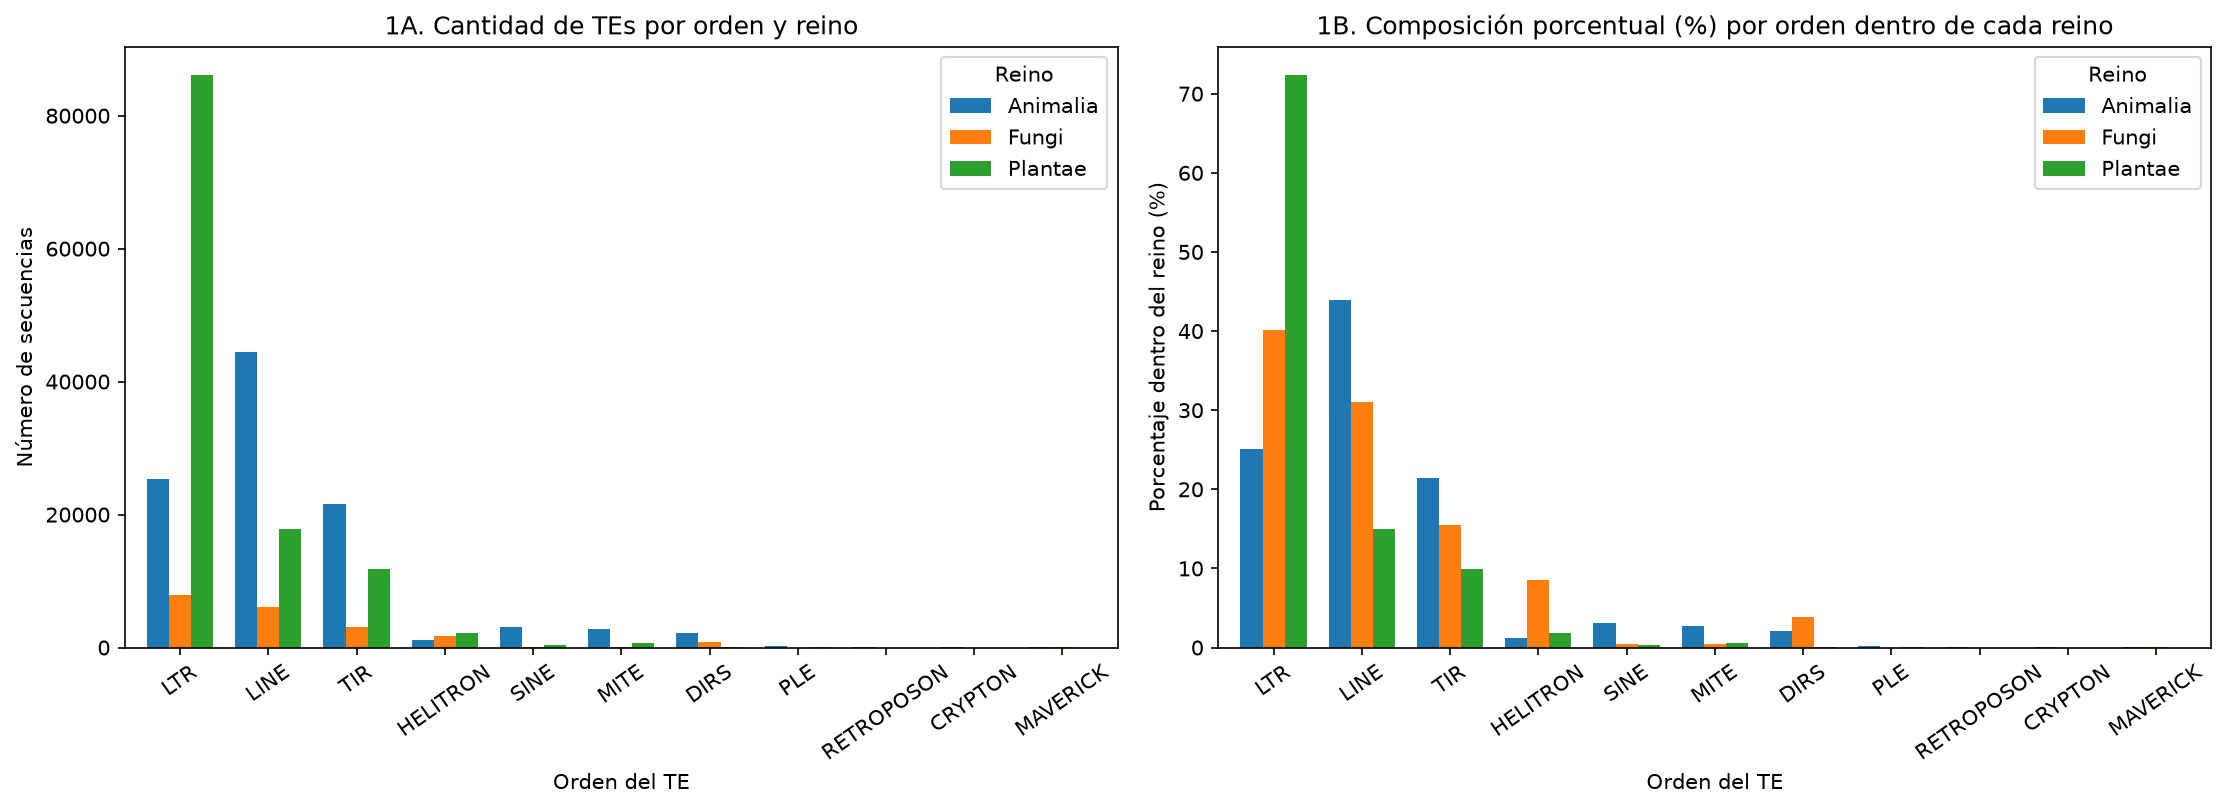
\includegraphics[width=\textwidth]{fig1_composicion_reino.png}
    \caption{Composición de la base de datos por reino.}
    \label{fig:reino}
\end{figure}

\begin{figure}[htbp]
    \centering
    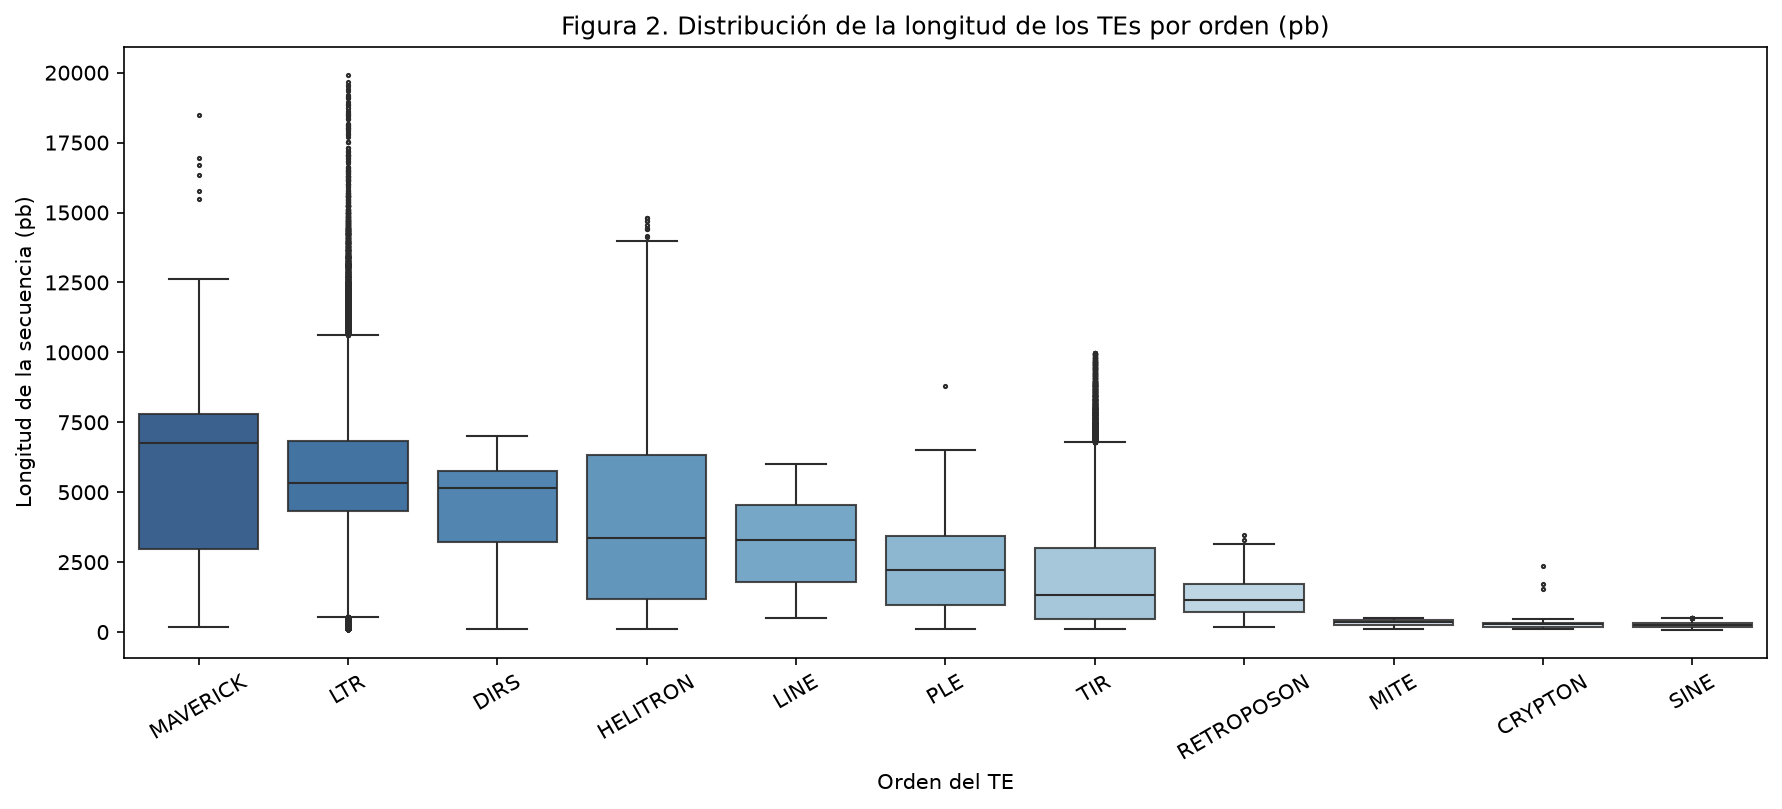
\includegraphics[width=\textwidth]{fig2_boxplot_longitud_orden.png}
    \caption{Longitud de las secuencias por orden de elemento transponible.}
    \label{fig:longitud}
\end{figure}

\begin{figure}[htbp]
    \centering
    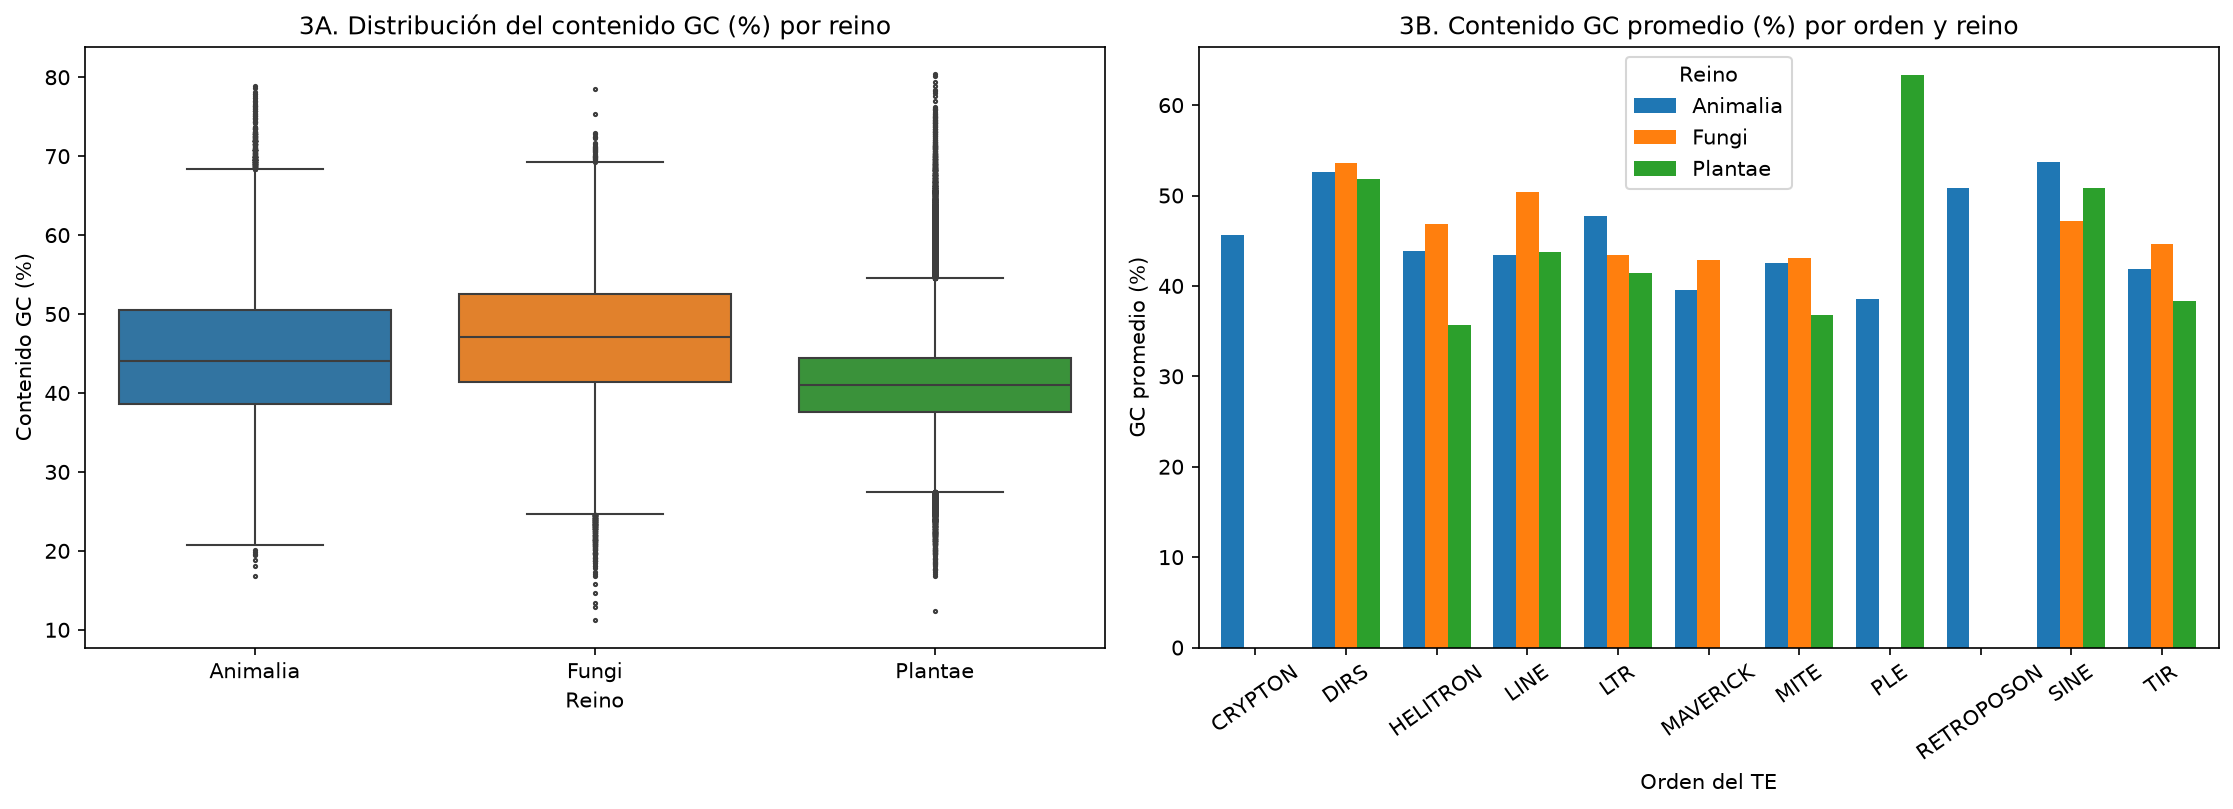
\includegraphics[width=\textwidth]{fig3_contenido_gc_reinos.png}
    \caption{Contenido de GC (\%) de las secuencias por reino.}
    \label{fig:gc}
\end{figure}

\begin{figure}[htbp]
    \centering
    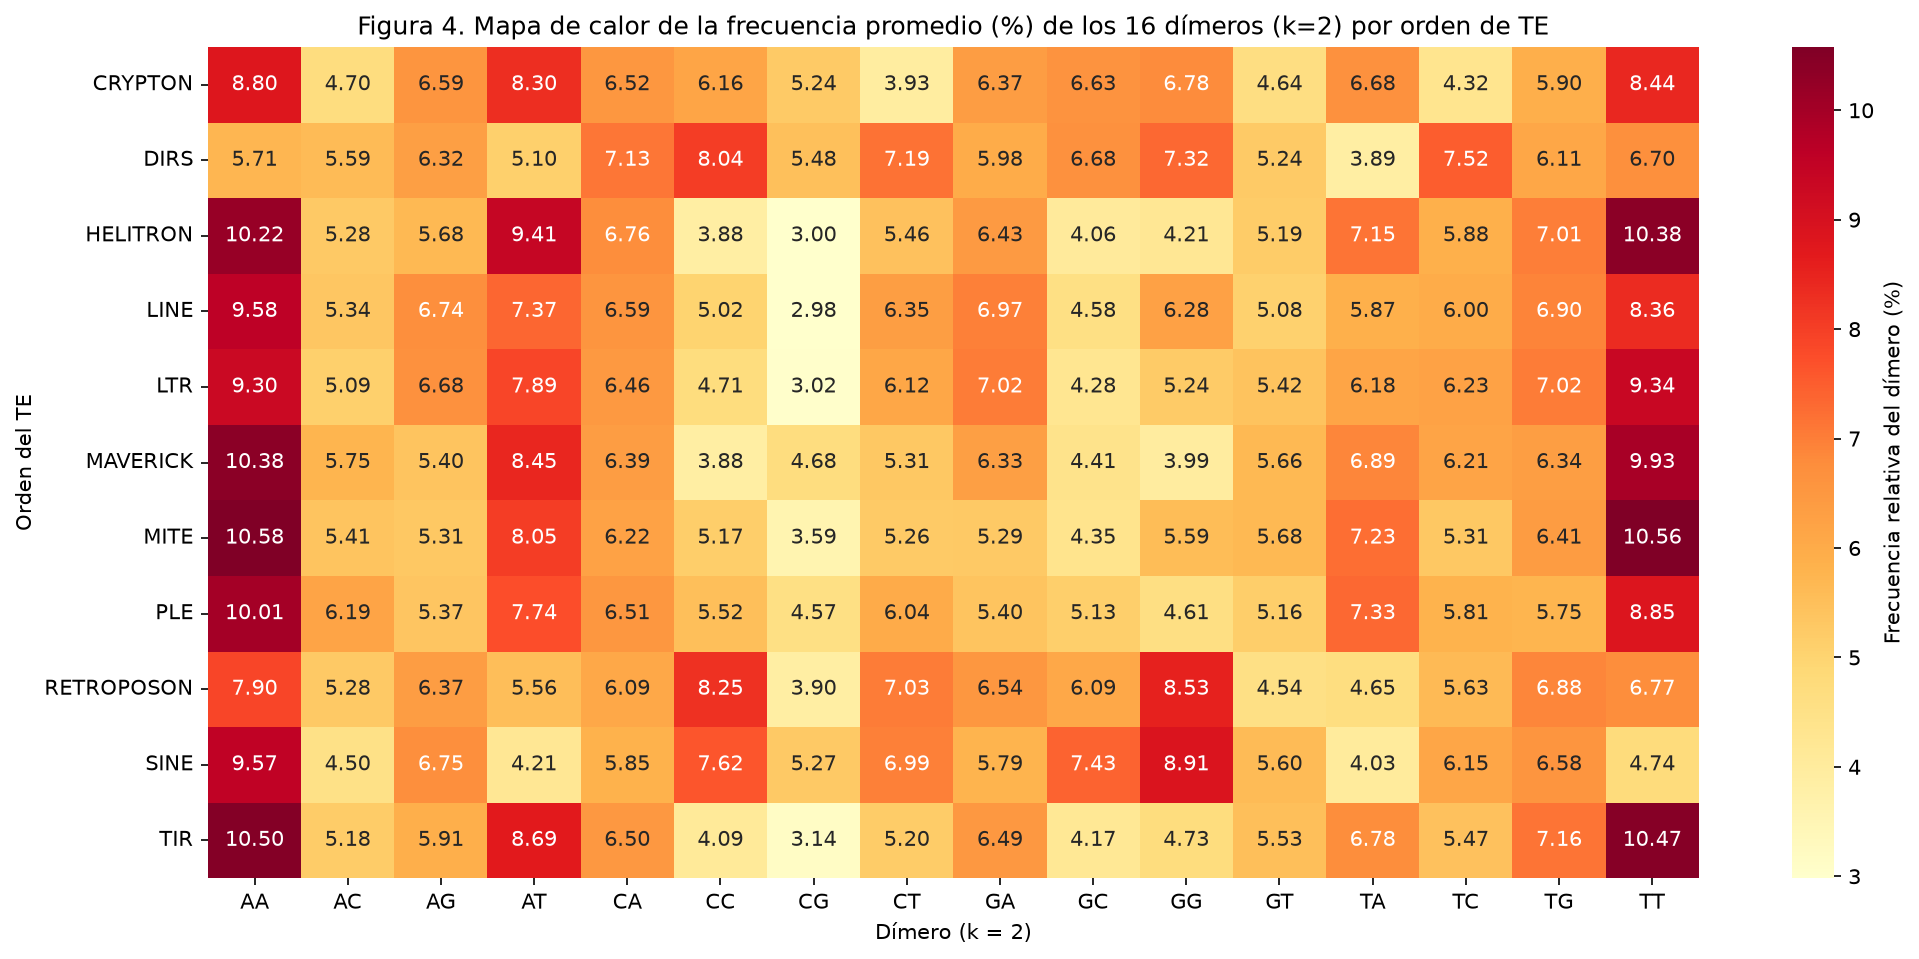
\includegraphics[width=\textwidth]{fig4_heatmap_kmers_k2.png}
    \caption{Mapa de calor de las frecuencias de dinucleótidos ($k=2$).}
    \label{fig:kmers}
\end{figure}

\subsection{Evaluación experimental de los diseños}\label{subsec:evaluacion}

Para cuantificar el rendimiento del diseño propuesto, se compararon dos arquitecturas de almacenamiento de k-mers (Estrategia A: k-mers embebidos; Estrategia B: k-mers separados en otra colección) y se midió el impacto de los índices estratégicos utilizando el comando \texttt{explain("executionStats")} de MongoDB. 

\textbf{Almacenamiento y tiempos de inserción.} La evaluación sobre una muestra de 20.000 secuencias reveló que el diccionario de k-mers representa aproximadamente el 90\% del peso del documento. En la Estrategia A, el documento promedio pesa 29,13 KB, ocupando 231,39 MB en disco. En la Estrategia B, la colección con metadatos (\textit{sequences\_light}) se redujo a 2,92 KB por documento (26,74 MB), mientras que los k-mers separados ocuparon 201,36 MB. Ambas estrategias demostraron tiempos de inserción idénticos ($\sim$12,7 segundos), evidenciando que el cuello de botella es el cálculo matemático en Python y no la escritura en base de datos. La proyección para las 239.946 secuencias indica un consumo en disco de aproximadamente 2,7 GB (Figura \ref{fig:comparativa}).

\textbf{Rendimiento de consultas analíticas vs. lectura directa.} Las consultas de agregación masiva que omiten los k-mers (como el cálculo de longitud promedio) se ejecutaron un 23\% más rápido en la Estrategia B, dado que el motor \textit{WiredTiger} descomprime bloques de datos 10 veces más ligeros. Sin embargo, para recuperar el perfil de k-mers junto con su taxonomía (necesario en bioinformática), la Estrategia A fue más eficiente (0,43 ms frente a 0,77 ms), ya que evita el costo del operador \texttt{\$lookup}.

\textbf{Impacto del indexado.} La validación de los índices creados sobre la base de datos completa demostró una aceleración de varios órdenes de magnitud (Figura \ref{fig:comparativa}). Una búsqueda puntual por \textit{sequence\_id} o un filtro compuesto (especie y superfamilia) utilizando un índice (\textit{IXSCAN}) retornó los datos en 0,35--0,37 ms examinando 1 o 2 documentos. Al forzar un escaneo completo (\textit{COLLSCAN}), el tiempo de respuesta ascendió hasta 117--153 ms, obligando al sistema a cargar y evaluar los 239.946 documentos.

\begin{figure}[htbp]
    \centering
    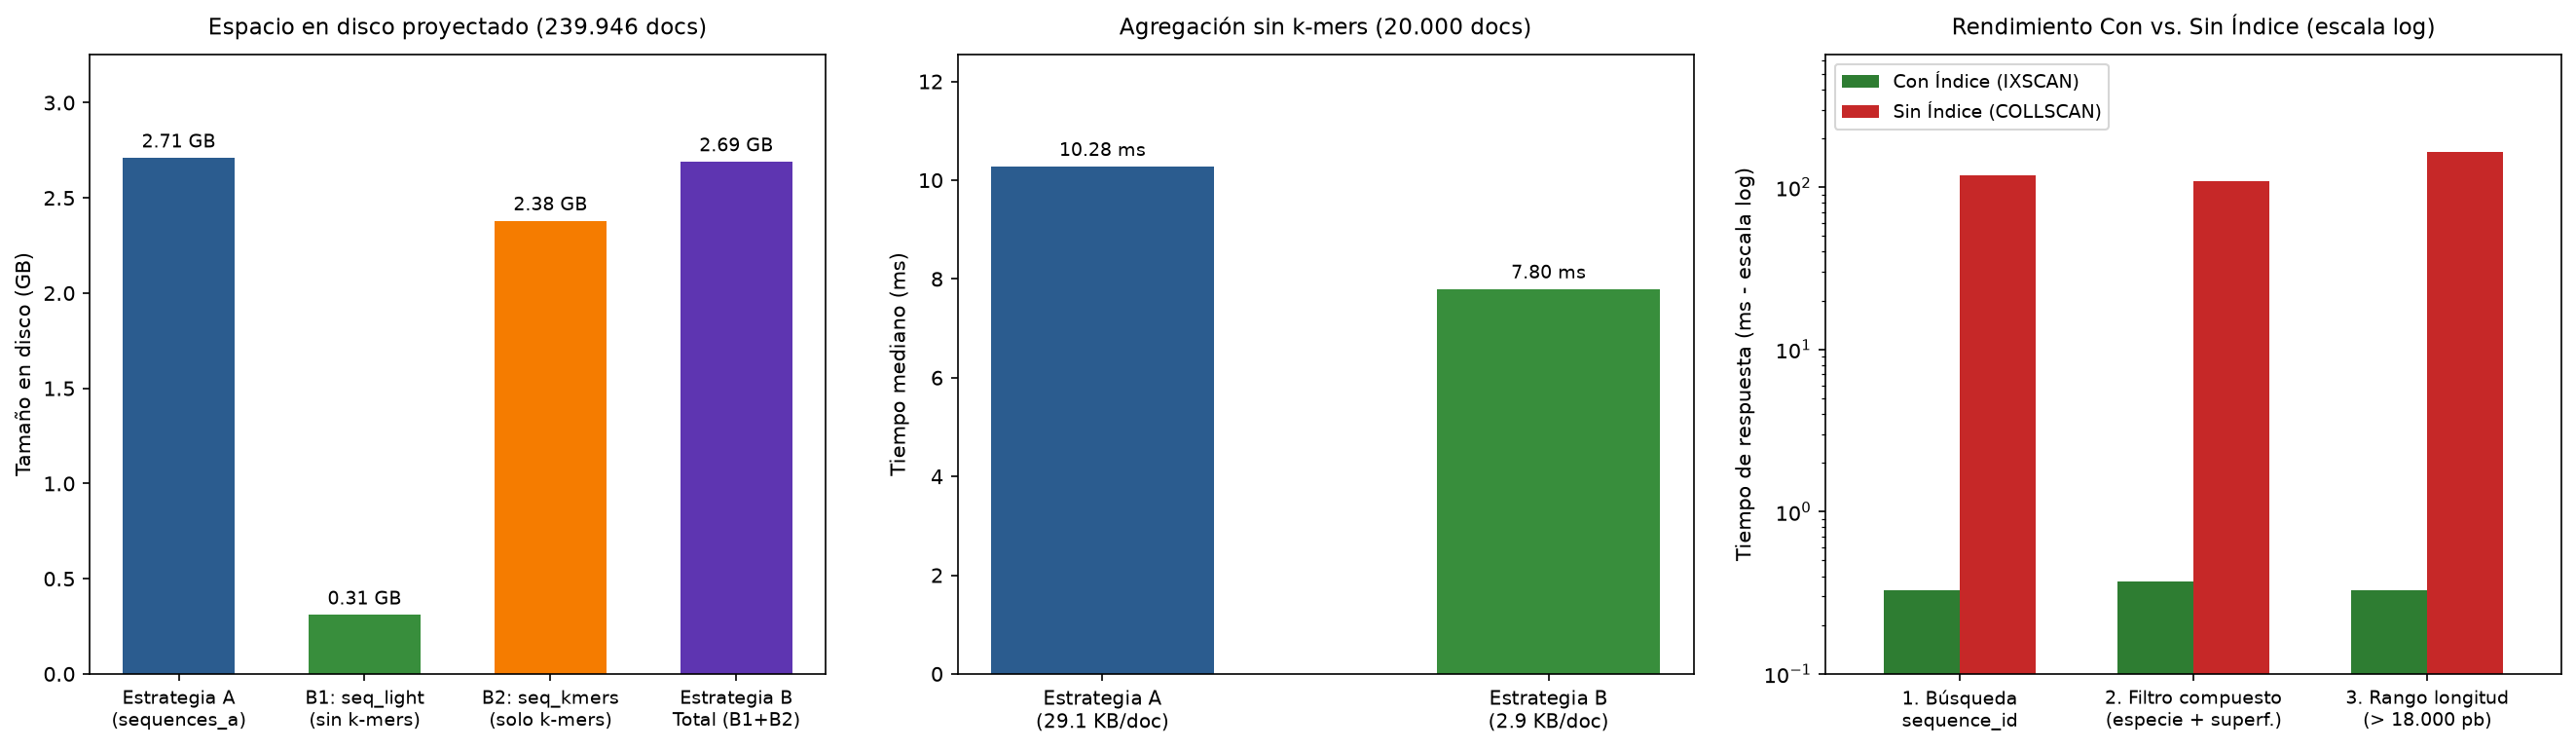
\includegraphics[width=\textwidth]{fase9_comparativa_experimental.png}
    \caption{Evaluación experimental: Espacio en disco proyectado, tiempo mediano de agregación sin k-mers (Estrategia A vs. B) y rendimiento logarítmico con índices frente a escaneo secuencial.}
    \label{fig:comparativa}
\end{figure}

\subsection{Ventajas y limitaciones del diseño}\label{subsec:limitaciones}

El diseño híbrido adoptado (taxonomía referenciada y características embebidas) presenta ventajas significativas para la consistencia y la velocidad de lectura. La inclusión de un esquema de validación estricto (\texttt{\$jsonSchema}) garantiza la integridad de los tipos de datos (como el control del enumerador en \textit{Kingdom}). Además, la normalización de la llave \textit{species\_key} eliminó los problemas de nomenclatura cruzada entre archivos. 

La principal limitación radica en el modelo de la Estrategia A para cargas de trabajo puramente analíticas (OLAP). Al mantener los diccionarios de k-mers embebidos, cualquier agregación sobre metadatos penaliza la memoria RAM al cargar información genética innecesaria para ese contexto.

\subsection{Crecimiento de los datos}\label{subsec:crecimiento}

Si el volumen de secuencias creciera 10 o 100 veces (alcanzando los 24 millones de registros y cientos de gigabytes), el esquema actual en un solo servidor de MongoDB agotaría la memoria RAM disponible para los índices y el \textit{cache} de \textit{WiredTiger}. 

Para soportar dicho crecimiento, la arquitectura debería migrar a un \textit{Sharded Cluster} de MongoDB. Se propondría fragmentar los datos (Sharding) utilizando una \textit{shard key} compuesta basada en \textit{species\_key} o \textit{te\_order}, lo que garantizaría una distribución uniforme y permitiría consultas locales por taxonomía. Asimismo, la \textbf{Estrategia B} (separación de k-mers) se volvería obligatoria, aislando las colecciones pesadas en fragmentos físicos independientes para no saturar las operaciones sobre los metadatos.

\subsection{Amenazas a la validez}\label{subsec:validez}

La validez del modelo depende de la calidad inherente de los datos de entrada en PanTEon Database. Durante la ingesta, se documentaron amenazas originadas por la heterogeneidad de las fuentes (Dfam y RM2+MCH):
\begin{itemize}
    \item \textbf{Incompletitud taxonómica:} El archivo de metadatos carecía de clasificación en 3 registros para Phylum, 49 para Clase y 76 para Familia, requiriendo el uso del tipo \texttt{null} en la validación \texttt{BSON} para evitar el rechazo de secuencias válidas.
    \item \textbf{Consistencia de Identificadores:} Un total de 31.600 secuencias no contaban con el prefijo estandarizado \textit{PDB} en el FASTA, utilizando en su lugar la nomenclatura nativa de la fuente de origen.
    \item \textbf{Calidad de Ensamblaje:} Se identificaron 4.374 secuencias con un porcentaje de nucleótidos indeterminados (\textit{N}) superior al 5\%, lo que introduce ruido estadístico en el cálculo de frecuencias relativas si no se excluyen las ventanas de lectura ambiguas en el \textit{pipeline}.
\end{itemize}

\section{Conclusiones}\label{sec:conclusiones}

El presente trabajo demostró la viabilidad de utilizar MongoDB como solución centralizada para almacenar, estructurar y analizar grandes volúmenes de elementos transponibles. El \textit{pipeline} desarrollado en Python logró la integración exitosa y reproducible de 239.946 secuencias heterogéneas procedentes de FASTA y metadatos taxonómicos de CSV. El modelo de datos, enriquecido con validaciones estrictas e índices estratégicos, resolvió eficientemente el reto de escalabilidad espacial derivado del almacenamiento de perfiles de k-mers, optimizando las consultas bioinformáticas. Los análisis experimentales respaldan que una arquitectura orientada a documentos es altamente competitiva para gestionar bibliotecas moleculares complejas, sirviendo como base estructural sólida para futuros desarrollos en \textit{machine learning} genómico.

\backmatter

\section*{Lista de abreviaturas}

\noindent ADN: ácido desoxirribonucleico; ARN: ácido ribonucleico; BSON: \emph{Binary JSON}; CSV: valores separados por comas; FASTA: formato de texto para secuencias biológicas; GC: guanina y citosina; OLAP: procesamiento analítico en línea; RAM: memoria de acceso aleatorio; TE: elemento transponible (\emph{transposable element}).

\section*{Declaraciones}

\bmhead{Aprobación ética y consentimiento para participar} No aplica.

\bmhead{Consentimiento para la publicación} No aplica.

\bmhead{Disponibilidad de datos y materiales} El código del \emph{pipeline}, los cuadernos y las figuras están disponibles en \url{https://github.com/JuanSebastianLopez15/Corte2Proyecto} (fecha de acceso: 29 de octubre de 2026). Los datos de PanTEon Database v1.6.1 se encuentran en Zenodo, \url{https://doi.org/10.5281/zenodo.19372616} (fecha de acceso: 29 de octubre de 2026) \cite{orozco2026panteondb}. El marco PanTEon se describe en \cite{orozco2026panteon}.

\bmhead{Conflictos de interés} Los autores declaran que no tienen conflictos de interés.

\bmhead{Financiación} Este trabajo no recibió financiación específica.

\bmhead{Contribuciones de los autores} Pendiente.

\bmhead{Agradecimientos} Los autores agradecen al profesor Simón Gaviria Orrego por la orientación en la asignatura Bases de Datos II de la Universidad Autónoma de Manizales.

\bmhead{Información de los autores} Estudiantes de Ingeniería de Sistemas de la Universidad Autónoma de Manizales, Colombia.


%%=============================================%%
%% For submissions to Nature Portfolio Journals %%
%% please use the heading ``Extended Data''.   %%
%%=============================================%%

%%=============================================================%%
%% Sample for another appendix section			       %%
%%=============================================================%%

%% \section{Example of another appendix section}\label{secA2}%
%% Appendices may be used for helpful, supporting or essential material that would otherwise 
%% clutter, break up or be distracting to the text. Appendices can consist of sections, figures, 
%% tables and equations etc.

%%===========================================================================================%%
%% If you are submitting to one of the Nature Portfolio journals, using the eJP submission   %%
%% system, please include the references within the manuscript file itself. You may do this  %%
%% by copying the reference list from your .bbl file, paste it into the main manuscript .tex %%
%% file, and delete the associated \verb+\bibliography+ commands.                            %%
%%===========================================================================================%%

\bibliography{sn-bibliography}% common bib file
%% if required, the content of .bbl file can be included here once bbl is generated
%%\input sn-article.bbl

\end{document}